\documentclass[10pt,a4paper]{ddedoc}

\usepackage{graphics,graphicx}
\usepackage{amsmath,amssymb}
\usepackage{url}
\usepackage{listings}

\pagestyle{plain}

\textwidth=6.25in
\textheight=9.5in
\hoffset=-0.6in
\voffset=-0.8in


\newcommand{\ds}{\displaystyle}

\newcommand{\fun}[1]{{\lstinline!#1!}}

\newcommand{\funp}[1]{{\tt #1}}

% A font for UNIX commands
\newcommand{\commandf}[1]{{\tt #1}}

% A font for environment variables
\newcommand{\envf}[1]{{\it #1}}

% A font for function names
\newcommand{\funcf}[1]{{\bf #1}}

% A font for filenames
\newcommand{\filef}[1]{{\sf #1}}

% A font for ftp sites and web pages
\newcommand{\webf}[1]{{\sl #1}}


% \def\knut{{P\kern-.15emD\kern-.15emD\kern-.15emE\raisebox{.25ex}{-}C\kern-.1emO\kern-.1emN\kern-.05emT}}
\def\knut{Knut}

\newcommand{\iconAdd}{\protect
\includegraphics[height=0.8\baselineskip]{fig/cr32-action-add}}
\newcommand{\iconEraser}{\protect
\includegraphics[height=0.8\baselineskip]{fig/cr32-action-eraser}}
\newcommand{\iconPrint}{\protect
\includegraphics[height=0.8\baselineskip]{fig/cr32-action-fileprint}}
\newcommand{\iconRun}{\protect
\includegraphics[height=0.8\baselineskip]{fig/cr32-action-launch}}
\newcommand{\iconStop}{\protect
\includegraphics[height=0.8\baselineskip]{fig/cr32-action-stop}}
\newcommand{\iconBuild}{\protect
\includegraphics[height=0.8\baselineskip]{fig/cr32-action-build}}
%\newcommand{\iconExit}{\protect
\includegraphics[height=0.8\baselineskip]{fig/cr32-action-exit}}
\newcommand{\iconSaveAs}{\protect
\includegraphics[height=0.8\baselineskip]{fig/cr32-action-filesaveas}}
\newcommand{\iconPencil}{\protect
\includegraphics[height=0.8\baselineskip]{fig/cr32-action-pencil}}
\newcommand{\iconText}{\protect
\includegraphics[height=0.8\baselineskip]{fig/cr32-action-view_text}}
\newcommand{\iconColorize}{\protect
\includegraphics[height=0.8\baselineskip]{fig/cr32-action-colorize}}
\newcommand{\iconOpen}{\protect
\includegraphics[height=0.8\baselineskip]{fig/cr32-action-fileopen}}
\newcommand{\iconSave}{\protect
\includegraphics[height=0.8\baselineskip]{fig/cr32-action-filesave}}
\newcommand{\iconRemove}{\protect
\includegraphics[height=0.8\baselineskip]{fig/cr32-action-remove}}
\newcommand{\iconSvg}{\protect\includegraphics[height=0.8\baselineskip]{fig/cr32-svg-export}}

\usepackage{tikz}
\newcommand{\dittotikz}{%
    \tikz{
        \draw [line width=0.12ex] (-0.2ex,0) -- +(0,0.8ex)
            (0.2ex,0) -- +(0,0.8ex);
        \draw [line width=0.08ex] (-0.6ex,0.4ex) -- +(-1.5em,0)
            (0.6ex,0.4ex) -- +(1.5em,0);
    }%
}

\begin{document}
\lstset{language=C++,tabsize=3,columns=flexible,breaklines=true,escapechar=\%}
\makeatother
%
\title{\knut{}}
\subtitle{A continuation and bifurcation software for delay-differential
equations}
\author{R\'obert Szalai}
\newcommand{\knutver}{5}
\version{\knutver}
\date{6 August 2012}
\maketitle

\begin{center}
{\bf \large Revision history } \vskip 0.25em
  \begin{tabular}{ |l|c|l| }
    \hline Date & Version & Institution \\
    \hline Sept.\ 2002 -- Jan.\ 2004 & & Budapest University of Technology and
Economics \\
    \hline Febr.\ 2004 -- July 2004 & & University of Bristol \\
    \hline Sept.\ 2004 -- June 2005 & 0.9.2 -- 0.9.8 & Massachusetts Institute
of Technology \\
    \hline July 2005 -- Sept. 2005 & 0.9.9 -- 0.9.17 & N.A. \\
    \hline 27 December 2005 & 0.9.21 (r83) & Budapest University of Technology and Economics \\
    \hline 16 March 2006 & 1.0.1 (r119) & Budapest University of Technology and Economics \\
    \hline 16 May 2006 & 1.0.2 (r139) & University of Bristol \\
    \hline 19 June 2006 & 1.0.3 (r153) & \dittotikz \\
    \hline 24 September 2006 & 1.1.0 (r245) & \dittotikz \\
    \hline 10 October 2006 & 1.1.1 (r260) & \dittotikz \\
    \hline 24 December 2006 & 1.1.2 (r315) & \dittotikz \\
    \hline 4 August 2007 & 1.1.3 (r343) & \dittotikz \\
    \hline 14 March 2008 & 1.2.0 (?) & \dittotikz \\
    \hline 13 March 2012 & 4 (?) & \dittotikz \\
    \hline
  \end{tabular}
\end{center}

\vskip 3em
\hrule
\vskip 2em
\begin{center} {\bf \large Trademarks } \vskip 0.25em \end{center}
The product names used in this manual are for identification purposes only. All
trademarks and registered trademarks are the property of their respective
owners.

\newpage

\tableofcontents

\newpage

\section{Introduction}

The software can analyze periodic orbits of delay-differential equations in the
general form
\begin{equation}
	\dot{x}(t) = f (t, x(t-\tau_0), x(t - \tau_1), \dots , x(t - \tau_r), \lambda
), \label{gensys}
\end{equation}
where $f$ can be either periodic in $t$ or independent of $t$, which is called
the autonomous case. The right hand side of (\ref{gensys}) and the delays
($\tau_i : \mathbb{R}^p \to [0,h)$ with $h<\infty$) smoothly depend on the
parameter vector $\lambda \in \mathbb{R}^p$. The solution $x(t)$ is assumed to
be an $\mathbb{R}^n$ valued continuous function satisfying the periodicity
condition
\[
	x(t) = x(t+T),\quad t \in \mathbb{R}.
\]
Because of periodicity, the software is tracking a function segment $\varphi \in
C([0,T],\mathbb{R}^n)$ only. The solution segment $\varphi$ is approximated by
piecewise polynomials \cite{engcol,engstab}.

The software can continue periodic orbits of (\ref{gensys}) along one scalar
parameter. It can determine the stability of a periodic orbit by computing
finitely many Floquet multipliers of the largest magnitude. Codimension-one
bifurcations are detected along the solution branch using the Floquet
multipliers, and bifurcation points can be calculated using test-functionals.
When a branching point of periodic orbits is encountered the software can be
directed to continue the other branch. Similarly, when a period doubling
bifurcation point is found, the period-two branch can be selected for
continuation.

The three generic codimension-one bifurcations (Neimark-Sacker, period doubling
and fold) can be continued along two parameters. The defining systems of these
bifurcations are minimally extended and use test-functionals. Moreover, a
limited number of codimension-two bifurcations can be continued, when two
different test-functionals are selected.

Equilibria of autonomous systems can also be continued as constant periodic
orbits with fixed period. In this case the Hopf bifurcation is detected as
Neimark-Sacker bifurcation, and the periodic solution, emanating from the Hopf
point, can be continued by switching to the periodic solution branch.
Although, continuing equilibria in this way is very inefficient, it might help
in avoiding the hassle of producing starting points using some other numerical
package like DDE-BIFTOOL \cite{DDEBIF} or simulation.

\section{Installation}

It is recommended to install the software from the source. This requires several freely
available development tools. For Microsoft Windows there is a self-extracting installer
available as well.

\subsection{Requirements of compiling the software}

For building and configuring the software the CMake\footnote{\url{http://www.cmake.org}}
utility is used. It is available for various operating systems. For compiling 
the software the GNU GCC C++ compiler\footnote{\url{http://gcc.gnu.org}} starting with 
version 4.6.3 is recommended.

The package uses the ATLAS\footnote{\url{http://math-atlas.sourceforge.net}}
basic linear algebra software library for matrix-vector operations. This library can be
tuned for the target processor, which takes a substantial amount of time.
To avoid the lengthy compilation it is possible to download
pre-compiled versions, which contain the necessary files (\filef{libatlas.a} and
\filef{libcblas.a}). When configuring the software CMake looks for these two files
in the \filef{ATLAS/lib} subdirectory of the source tree, \filef{/usr/lib}, \filef{/usr/lib/atlas} 
and some additional directories in this order.

The (optional) graphical user interface requires the Qt\footnote{\url{http://www.trolltech.com}} 
toolkit (version 4.8). CMake looks for the \filef{qmake} utility to find the Qt
installation, so make sure that \filef{qmake} is in your \filef{\$PATH}.

\subsection{Linux and Unix}

The software comes in a compressed source archive form
\filef{Knut-{\knutver}.tar.bz2}, so it has to be uncompressed first into a
convenient directory using the following command:
{ \small \begin{quote} \begin{lstlisting}[basicstyle=\ttfamily,frame=single]
$ bzip2 -d Knut-%\knutver%.tar.bz2
$ tar xvf Knut-%\knutver%.tar
\end{lstlisting} \end{quote} } \noindent
The second step is to copy the compiled ATLAS library files (\filef{libatlas.a}
and \filef{libcblas.a}) into the
\filef{Knut-\knutver/ATLAS/lib} subdirectory.

Now the package is ready for the automatic configuration:
{ \small \begin{quote} \begin{lstlisting}[basicstyle=\tt,frame=single]
$ cd Knut-%\knutver%
$ ./build-unix.sh
\end{lstlisting} \end{quote} } \noindent
This configures and builds software after which it installs into the
\filef{knut/} folder in the user's home directory.
In order to make the software work, the \filef{PATH} environment variable has
to be set up. In the case of the \filef{bash} shell include the
{ \small \begin{quote} \begin{lstlisting}[basicstyle=\tt,frame=single]
export PATH=$PATH:$HOME/Knut/bin
\end{lstlisting} \end{quote} } \noindent
line into the \filef{.bash\_profile} configuration file in your \filef{HOME}
directory. For the C shell (\filef{csh}) insert the following line
{ \small \begin{quote} \begin{lstlisting}[basicstyle=\tt,frame=single]
setenv PATH $PATH:$HOME/Knut/bin
\end{lstlisting} \end{quote} } \noindent
into \filef{.cshrc}. To activate the changes log out and log in again.

\subsection{Windows}

The simplest way of installing the software is to run the
\filef{Knut-{\knutver}.exe}, which will extract the package into a
preferred directory and set up a \filef{Start Menu} shortcut.

Cross compilation is also possible on a Linux system using MinGW cross compiler toolchain. 
The following command will create a package
{ \small \begin{quote} \begin{lstlisting}[basicstyle=\tt,frame=single]
build-win-cross.sh
\end{lstlisting} \end{quote} } \noindent

\section{Command line inferface (CLI)}

The software is controlled by the so-called \emph{constants file}. It is an XML file
that contains instructions about all the operations done by the software and
also specifies the parameters of the numerical method.
The name of a constants file can be given to the software using the \funp{-c} option.
The syntax of the command line arguments is illustrated as
{ \small \begin{quote} \begin{lstlisting}[basicstyle=\tt,frame=single]
$ knut -c <constants-file> 
\end{lstlisting} \end{quote} } \noindent
To display version information use the \funp{-v} command line switch.
{ \small \begin{quote} \begin{lstlisting}[basicstyle=\tt,frame=single]
$ knut -v
This is Knut version 4 (502, Fri Aug 3 14:33:57 2012 +0100, 19bc64e462a1e1793362eaf2c5d7f29c2d04dbd5)
\end{lstlisting} \end{quote} } \noindent


\subsection{The constants file}
\label{constfile}

As an example, we included the constants file of a laser system:
{ \small \begin{quote} \begin{lstlisting}[basicstyle=\tt,frame=single]
<?xml version="cfile 1.0" encoding="utf-8"?>
<knut version="5"> <branch input="" output="out-start.mat"
sysname="laser.vf" fromtype="NX" label="0" pointtype="USER" cp="eta"
switch="NX" eqns="DDE_LC,PHASE_ROT" vars="DDE_LC,bb" nint="20" ndeg="5"
nmul="20" stab="1" curvature="0.25" nint1="12" nint2="12" ndeg1="4"
ndeg2="4" steps="15" iad="0" npr="10" cpmin="-100" cpmax="100"
ds="-0.002" dsmin="0.0002" dsmax="0.002" dsstart="0.02" epsc="1e-05"
epsr="1e-05" epsk="1e-06" nitc="22" nitr="12" nitk="22" nderi="8"
symre="0,3" symim="1,4" />
</knut>
\end{lstlisting} \end{quote} } \noindent
This file corresponds to continuation of equilibria. The meaning of the
parameters are as follows.
\begin{description}
\item[\funp{input}] ~\\
A MATLAB v4 \filef{.mat} file as input, produced in previous runs.
\item[\funp{output}] ~\\
A MATLAB v4 \filef{.mat} to be written as an output.
\item[\funp{sysname}] ~\\
The name of the the system definition file, which can be a C++ file (\filef{.cpp}), a shared object (\filef{.so}) or a vector field file (\filef{.vf}). The type of the file is automatically detectedm but it can also be specified by the \funp{type} attribute. The value of the type attibute can be \funp{type="so"} for shared object code, \funp{type="cpp"} for C++ definition, \funp{type="vf"} vector field file to be compiled to shared object or \funp{type="vf0"} if no compiler is available on the system. The recommended format is the vector field file.
%
\item[\funp{fromtype}] ~\\\
The type of the solution to look for in the input file. 
\funp{NX}: any solution; \funp{NS} Neimark-Sacker bifurcation point; \funp{PD} period doubling; \funp{EP} the last point of the input.
%
\item[\funp{label}] ~\\
The \funp{label}th solution label in the input file, e.g., the 3rd Neimark-Sacker bifurcation. The program continues this
solution. If \funp{label}=0 it uses the starting solution specified 
in the system definition file.
%
\item[\funp{pointtype}] ~\\
Specifies the type of the solution to be continued. It can be one of the following numbers.
The number surrounded by parantheses refers to how many additional free
parameters are required.

Algorithms for time-periodic (non-autonomous) systems:
\begin{description}
\item[\funp{DDE\_LC} -] Continuation of periodic solutions. (0)
%
\item[\funp{DDE\_LP} -] Continuation of fold bifurcations in two parameters (1). The
input is a periodic solution at a fold bifurcation point. The software first
generates a starting point, that is, it tries to converge to the fold point. After the fold point is found with a good accuracy (see
\funp{EPSR}), the tangent of the fold curve is computed so that the continuation
can start. All the bifurcations are started in this way.
%
\item[\funp{DDE\_PD} -] Continuation of period doubling bifurcations. (1)
%
\item[\funp{DDE\_NS} -] Continuation of Neimark-Sacker (secondary Hopf) bifurcations.
(1)
%
\item[\funp{DDE\_BP\_SW} -] The software switches to the other solution at a branching point and
follows the new branch. Similar to \funp{TYPE=41}, first the software converges to
the critical solution. Then it computes the critical eigenfunction
$\varphi^{cr}$, which will become the tangent of the new branch, so that the
continuation can start. (0)
%
\item[\funp{DDE\_PD\_SW} -] The software first switches to the period-two branch at a
period doubling bifurcation point
(-1 multiplier) and then follows the new branch. The internal parameter \funp{I0} is multiplied by two. (0)
\end{description}
In the case of autonomous systems the above continuations can be carried out in
the same way. The important difference is that the software will use a phase
condition and continue an additional free parameter (e.g., the period). When a
fold bifurcation is continued a different test functional is used to account for
the trivial +1 Floquet multiplier of a periodic orbit.
\begin{description}
\item[\funp{DDE\_AUT} -] Continuation of periodic solutions in autonomous systems. The
additional parameter is usually the period length \funp{T}. (1)
%
\item[\funp{DDE\_AUT\_LP} -] Continuation of fold bifurcations in two parameters. (2)
%
\item[\funp{DDE\_AUT\_PD} -] Continuation of period doubling bifurcations. (2)
%
\item[\funp{DDE\_AUT\_NS} -] Continuation of Neimark-Sacker (secondary Hopf) bifurcations.
(2)
%
\item[\funp{DDE\_AUT\_BP\_SW} -] Switches to the other solution branch at a branching point and
follows the periodic orbits. (1)
%
\item[\funp{DDE\_AUT\_PD\_SW} -] The software first switches to the period-two branch at a
period doubling bifurcation point
(-1 multiplier) and then follows the arising orbits. (1)
%
\item[\funp{DDE\_AUT\_HOPF\_SW} -] Switches to the periodic solution branch arising at a Hopf
bifurcation point. The input is a constant solution, which represents a fixed
point. The failure or success of the switch depends on the choice of the period
length for the fixed point and the starting solution amplitude \funp{dsstart}.
As a rule of thumb, the period of the constant solution should be chosen as
small as possible to reliably detect the period of the arising periodic orbit.
If chosen period is too large, the period on the new branch will not be reliably detected. 
Therefore, the software will not be able to find the new branch. The software will warn 
the user if this is the case. (1)
\end{description}
The software can also continue invariant tori arising at Neimark-Sacker
bifurcation points. To continue these quasi-periodic orbits use the following
parameters when restarting from Neimark-Sacker points. This is an experimental
feature and  it is tested for non-autonomous systems only. The output has a different format
than specified in section \ref{matformat}, but it can be plotted using the matlab script 
\filef{matlab/torplot.m}.
\begin{description}
\item[\funp{DDE\_TORUS} -] Continuation of tori in time-periodic systems. Start from a torus in the input file.
\item[\funp{DDE\_TORUS\_SW} -] Start at a Neimark-Sacker bifurcation point.
%
\item[\funp{DDE\_AUT\_TORUS} -] Continuation of tori in autonomous systems. Start from a torus in the input file.
\item[\funp{DDE\_AUT\_TORUS\_SW} -] Start at a Neimark-Sacker bifurcation point.
\end{description}
If none of the above applies to a problem, it is possible to specify the set of
equations and variables used in continuation, by setting the \funp{pointtype} to
\funp{USER}.
%
\item[\funp{cp}] ~\\
It defines the main continuation parameter as it is named in the vector field file. Internal parameters can also be selected:
\begin{description}
\item[\funp{PAR\_ANGLE} -] represents the argument of the characteristic multiplier in the case of
Neimark-Sacker bifurcation continuation.
\item[\funp{PAR\_PERIOD} -] It is initialized to 1.0 when \funp{LABEL}=0. It doubles with
every period doubling branch switch (\funp{TYPE=45,55}). Use this as \fun{par(sys_npar()+1)} in the
system definition to rescale the delay or adjust the forcing if necessary. (See \filef{demo/tq} as an example.)
\item[\funp{PAR\_ROT\_NUM} -] contains the rotation number of a two-torus. Usually this is kept
constant in order to avoid strong resonances.
\end{description}
%
\item[\funp{switch}] ~\\
Branch swithing to be performed for user defined equations.
\begin{description}
\item[\funp{NX} -] No switch.
\item[\funp{BP} -] Switches to the other branch at a branching point. \funp{PAR\_PERIOD} is doubled.
\item[\funp{PD} -] Switches to the period-two branch at a period doubling
bifurcation.
\item[\funp{HOPF} -] Switches to the periodic solution branch at a Hopf
bifurcation.
\item[\funp{TORUS} -] Switches to a quasi-periodic torus at a Neimark-Sacker
bifurcation.
\item[\funp{AUT\_BP} -] branch switch for autonomous systems;
\item[\funp{AUT\_ROT\_BP} -] branch swithc for symmetric systems.
\end{description}
%
\item[\funp{parx}] ~\\
A comma separated list of parameter names specifying additional continuation parameters. In
the case of autonomous problems either \funp{cp} or this should include
\funp{T}, which refers to the period length. Note that internal parameters can also be used.
%
\item[\funp{eqns}] ~\\
For user defined systems, this contains the comma separated list of equations. Possible equations are:
\begin{description}
\item[\funp{NX} -] No equation is used.
\item[\funp{DDE\_LC} -] Periodic solution. This is always the first equation and can
only occur there.
\item[\funp{PHASE} -] Phase condition for autonomous systems.
\item[\funp{PHASE\_ROT} -] Phase condition for systems with additional symmetry. (For
details, see \cite{haegeman,roose-szalai}.)
\item[\funp{DDE\_TORUS} -] Quasiperiodic solution on a torus.
\item[\funp{TORUS\_PHS1} -] The first phase condition for the torus. This is applied
only in the case of autonomous equations.
\item[\funp{TORUS\_PHS2} -] The second phase condition for the torus. It is always
necessary.
\item[\funp{DDE\_TF\_LP} -] Test functional for fold bifurcations in forced systems.
\item[\funp{DDE\_TF\_PD} -] Test functional for period doubling bifurcations.
\item[\funp{DDE\_AUT\_TF\_LP} -] Test functional for fold bifurcations in autonomous systems.
\item[\funp{DDE\_AUT\_ROT\_TF\_LP} -] Test functional for fold bifurcations in autonomous systems
with symmetry. This is an experimental feature, probably will not work.
\item[\funp{DDE\_TF\_NS\_RE} -] Real part of the complex test functional for Neimark-Sacker
bifurcation.
\item[\funp{DDE\_TF\_NS\_IM} -] Imaginary part of the complex test functional for
Neimark-Sacker bifurcation. This imaginary part should directly follow the real
part in the list of equation, otherwise the software will not start the
continuation.
\end{description}
%
\item[\funp{vars}] ~\\
For user defined systems, this contains the comma separated list of variables. Possible variables are solution profiles, parameters and internal parameters. The code for solution profiles are. The internal parameters are detailed at the description of \funp{cp}.
\begin{description}
\item[\funp{NX} -] No variable is used.
\item[\funp{DDE\_LC} -] Periodic solution.
\item[\funp{DDE\_TORUS} -] Quasi-periodic solution.
\end{description}
%
\item[\funp{nint}] ~\\
Number of collocation intervals; heavily depends on the problem.
%
\item[\funp{ndeg}] ~\\
Degree of polynomials used in collocation. Usually 4 or 5. 
5 is recommended because superconvergence is lost for delay equations. Supported up to 25.
%
\item[\funp{nmul}] ~\\
The number of Floquet multipliers to be computed.
%
\item[\funp{stab}] ~\\
If zero, stability is not computed along the branch. In any case, \funp{nmul}
must have a reasonable value, because the eigenvalues are used when computing
the argument of the critical multiplier when starting a Neimark-Sacker
bifurcation continuation.
%
\item[\funp{nmat}] ~\\
This is the ratio of the maximum delay and the period length. More precisely, it
is the smallest integer such that $\funp{NMAT} \ge \tau_{MAX}/T_{MIN}$.
%
\item[\funp{steps}] ~\\
Maximum number of steps on the solution branch. The size of the output file is proportional to this number.
%
\item[\funp{iad}] ~\\
The software adapts the mesh after every \funp{IAD} continuation steps.
If \funp{iad}=0, no mesh adaptation will be performed. The recommended value is \funp{IAD}=3,
although in some cases it might be necessary to turn off the mesh adaptation.
Here, the same adaptation technique is used as in AUTO, hence, it is not optimal for delay equations. Nevertheless it is sufficiently good.
%
\item[\funp{npr}] ~\\
Print only every \funp{npr}th line.
%
\item[\funp{cpmin}, \funp{cpmax}] ~\\
These are the minimal and maximal values of the continuation parameter. The continuation stops if one them is reached.
%
\item[\funp{ds}] ~\\
Starting value of the stepsize in the pseudo-arclength continuation.
It should be reasonably small depending on the problem. \funp{ds} is adapted in
every continuation step between its minimum and maximum value. If the Newton
method exceeds \funp{nitc} iterations and \funp{ds} reached its minimum value,
the continuation is stopped.
%
\item[\funp{dsmin}, \funp{dsmax}] ~\\
The minimum and maximum values of \funp{ds}.
%
\item[\funp{dsstart}] ~\\
Specifies the $L^2$ distance of the first point on the new branch from the bifurcation 
point at branch switching (\funp{TYPE=20,30,44,45,54,55,56}).
%
\item[\funp{epsc}] ~\\
Tolerance of convergence to a periodic solution during continuation. For
periodic orbit continuation it is about $10^{-5} - 10^{-6}$, for continuation of
bifurcations it can be a bit larger about $10^{-4} - 10^{-5}$ to achieve
reasonable stepsizes (\funp{ds}).
%
\item[\funp{epsr}] ~\\
Tolerance in the refinement of periodic solutions. (Solution refinement is used
only before continuation starts.) It should be less than or equal to
\funp{epsc}. This constant is also used when finding bifurcation points.
%
\item[\funp{epsk}] ~\\
Tolerance when locating a singular vector of an operator. This is used when the initial tangent vector to a branch is sought,
and when a tangent vector is refined after adapting the mesh. It is also used for setting up a test functional for bifurcation continuation.
%
\item[\funp{nitc}] ~\\
Maximum number of Newton iteration steps within a continuation step.
%
\item[\funp{nitr}] ~\\
Maximum number of Newton iteration steps, when converging to an initial
solution.
%
\item[\funp{nitk}] ~\\
Maximum number of iteration steps, when locating a singular vector of an operator. (See \funp{epsk}.)
%
\item[\funp{nderi}] ~\\
The highest order of closed form derivatives to be used. If this number is low, finite difference derivatives will be used instead.
%
\item[\funp{symre}] ~\\
In case of symmetric systems, the comma separated list of indices of the real parts of the symmetric part of the solution.
%
\item[\funp{symim}] ~\\
In case of symmetric systems, the comma separated list of indices of the imaginary parts of the symmetric part of the solution.
\end{description}

\subsection{Input/output file format}
\label{matformat}

The software uses {\sc{}mat} files to store the results of continuation.
The inner structure of these files are documented in \cite{matfile}. 
These files can be read also by the GNU octave \cite{octave}.
A \knut{} {\sc{}mat} file contains several matrices, describing a branch of solutions.
The structure of these matrices are defined in Table \ref{matstruct}.
\begin{table}[bth!]
\begin{tabular}{|c|c|c|l|}
\hline
Matrix name & Rows & Columns & Content\\
\hline 
\funp{knut\_npoints} & 1 & 1 & \begin{minipage}[c]{0.4\linewidth} Number of points
computed in the branch of solutions. \end{minipage}\\
\hline
\funp{knut\_par} & \funp{npar}+3 & \funp{steps} & Values of parameters. \\
\hline
\funp{knut\_mul} & \funp{nmul} & \funp{steps} & The Floquet multipliers. \\
\hline
\funp{knut\_ntrivmul} & 1 & 1 & Number of trivial multipliers. \\
\hline
\funp{knut\_ndim} & 1 & \funp{steps} & \begin{minipage}[c]{0.4\linewidth}
\funp{ndim}: dimesion of the right-hand-side function $f$ \end{minipage}\\
\hline
\funp{knut\_elem} & \funp{ndeg}+1 & \funp{steps} & Mesh points in a collocation
interval. \\
\hline
\funp{knut\_mesh} & \funp{nint}+1 & \funp{steps} & Mesh points of the solution
profile. \\
\hline
\funp{knut\_prof} & \funp{ndim}$\times$(\funp{nint}$\times$\funp{ndeg}+1) &
\funp{steps} & The solution profile. \\
\hline
\end{tabular}
\caption{The contents of the {\sc{}mat} files.}
\label{matstruct}
\end{table}
If the computation stops for some reason, \funp{knut\_npoints} will be less than
\funp{STEPS}, but the size of the {\sc{}mat} file will not be smaller, so only the first
\funp{knut\_npoints} columns will contain valid data.

To convert the input and output {\sc{}mat} files to the format of DDE-BIFTOOL use the
\funp{pmat2branch.m} and \filef{branch2pmat.m} {\sc{}matlab} scripts found in the \filef{matlab}
subdirectory of the package. The function \funp{pmat2branch.m} takes only one 
input argument, which is the name of a Level 4 {\sc{}mat} file, and returns a periodic 
solution branch structure of DDE-BIFTOOL:
{ \small \begin{quote} \begin{lstlisting}[frame=single]
>> psbr = pmat2branch( 'input-file' );
\end{lstlisting} \end{quote} } \noindent
To export results out of DDE-BIFTOOL and produce a \knut{} {\sc{}mat} file, issue the command
{ \small \begin{quote} \begin{lstlisting}[frame=single]
>> branch2pmat( 'output-file', psbr, nmul );
\end{lstlisting} \end{quote} } \noindent
where \funp{NMUL} is the same number as in the constants file where the exported data 
will be used as a starting solution.

\subsection{Defining an equation}

Use vector field files as described at \url{http://www.warrenweckesser.net/vfgen/menu_fileformat.html}

\subsection{Running the software}

After invoking the software \filef{knut}, it either loads a solution profile
from the input file (see Sect.\ \ref{constfile}) or uses the 
\fun{sys_stpar} and \fun{sys_stsol} functions 
depending on the value of \funp{label} to obtain an approximate solution at a
given value of parameters. There are three steps of initializations before the
continuation starts:
\begin{enumerate}
\item The software starts a Newton iteration to converge to a more precise
solution.
\item If there is a bifurcation involved, e.g., in the case of a bifurcation
continuation or branch switching, the software tries to find the bifurcation
point using a Newton method. Clearly, if there is no bifurcation point in a
sufficiently small neighborhood of the specified solution, this step will fail.
In very rare cases and for `difficult' problems, if the first and second
derivatives of the right hand side are computed numerically (\fun{sys_nderi}
returns zero or one), the search for a bifurcation can fail even when the
starting solution is the bifurcation point with high accuracy.
\item The software finds the tangent of the solution branch at its first point. In
general, it computes the tangent as a kernel vector of the linearized defining
system. In the case of branch switching, the critical eigenfunctions are used to
construct the tangent vector.
\end{enumerate}
If any of the above tasks fail, or the convergence is not reached within the
specified number of steps and accuracy, the program stops.
After all this initializations, the program starts the continuation and writes
the data into the output and branch files.

\subsubsection{The console output}

First, the software writes the content of the constants file (see Sect.\
\ref{constfile}) to the standard output (console). Then it starts the Newton
iteration:
{ \small \begin{quote} \begin{lstlisting}[basicstyle=\tt,frame=single]
IT      ERR             SOLnorm         DIFFnorm
 0      5.772096e-02    9.234583e-01    1.110239e-01
 1      6.083138e-02    9.279196e-01    1.172780e-01
 2      1.271950e-02    9.283746e-01    2.452796e-02
 3      7.432386e-04    9.283646e-01    1.433235e-03
 4      1.490474e-06    9.283646e-01    2.874176e-06
\end{lstlisting} \end{quote} } \noindent
Here, each iteration step (\funp{IT}) is displayed: \funp{SOLnorm} is the $L^2$
norm of the solution and \funp{DIFFnorm} is the $L^2$ norm of the difference
between the new and the previous approximate solution. \funp{ERR} refers to the
stopping criterion, that is
\[
	\funp{ERR} = \frac{\funp{DIFFnorm}}{1+\funp{SOLnorm}} < \funp{EPSR}.
\]
If the prescribed accuracy is not reached, but \funp{IT} reaches \funp{NITR},
the program stops with error.

In the next step, if appropriate, the program tries to find the bifurcation
point. This is done by the same Newton method, so it will quickly converge if
the bifurcation point is sufficiently close:
{ \small \begin{quote} \begin{lstlisting}[basicstyle=\tt,frame=single]
--- Finding the bifurcation point (TF) ---

IT      ERR             SOLnorm         DIFFnorm
 0      3.521412e-04    9.141656e-01    6.740565e-04
 1      8.795736e-06    9.141643e-01    1.683648e-05
\end{lstlisting} \end{quote} } \noindent

The main continuation proceeds similarly:
{ \small \begin{quote} \begin{lstlisting}[basicstyle=\tt,frame=single]
LABEL      NORM         P2              P0              USTAB   IT
  1     9.142448e-01    1.556134e+00    1.101504e+01      0     2
  2     9.143658e-01    1.557164e+00    1.101898e+01      0     1
  3     9.144963e-01    1.558277e+00    1.102330e+01      0     1
\end{lstlisting} \end{quote} } \noindent
The first column, \funp{LABEL} is the solution label in the output file, and
the second column is the $L^2$ norm of the solution. From the third column on,
the free parameters are displayed. The column denoted by \funp{USTAB} refers to
the number of unstable characteristic roots, if stability computation is turned
on (see \funp{STAB} below), otherwise it is constantly zero regardless of the actual stability. 
The last column is the number of Newton iterations in a continuation step.

\subsection{Example: Mackey-Glass equation}

Here, we discuss the continuation steps in the case of a simple one dimensional
delay-differential equation. Although the equation is simple, it shows quite
complicated dynamics including chaos. Our equation reads
\begin{equation}
  \dot{x} ( t ) = ax ( t ) + b \frac{x ( t - \tau )}{1 + x^{10} ( t - \tau )}.
\label{ct:glass}
\end{equation}
This equation models proliferation of white blood cells and was first
introduced by Mackey and Glass in {\cite{mackey}}. Equation (\ref{ct:glass})
has three equilibrium solutions $x_1 = 0$ and $x_{2, 3} = \sqrt[10]{- ( a + b
) / a}$, which connect to each other at $a = - b$ by a supercritical pitchfork
bifurcation. The nonzero solutions can lose their stability through Hopf
bifurcation described by the parametric curves
\begin{align*}
  a & =-\arccos(-d^{-1}){\frac{1}{{\tau} {\sqrt[10]{d^2-1}}}}\\
  b & ={\frac{10a}{d-9}},
\end{align*}
where $|d| \ge 1$. Hopf bifurcations for $d > 1$ are supercritical, which give
rise to stable periodic orbits. These periodic orbits bifurcate further by
several period doublings leading to chaotic motion. It was demonstrated by
Hale and Sternberg {\cite{sternberg}} that chaos arises due to the transverse
intersection of the two-dimensional unstable and infinite dimensional stable
manifold of this periodic orbit.

The vector field file can be found in the directory \filef{demo/glass/mackey-glass.vf}. 
{ \small \begin{quote} \begin{lstlisting}[basicstyle=\tt,frame=single]
<?xml version="1.0"?>
<VectorField Name="mackey_glass">
<Parameter  Name="T"   DefaultValue="2.0" Description="Period" />
<Parameter  Name="a"   DefaultValue="-1.0" />
<Parameter  Name="b"   DefaultValue="1.5" />
<Parameter  Name="tau" DefaultValue="2.0" />
<Expression Name="DX"  Formula="delay(X,tau)" />
<StateVariable Name="X" 
  Formula="a*X + b*DX/(1+DX^10)"
  DefaultInitialCondition="((1.0-1.5)/(-1.0))^(1.0/10.0)" DefaultHistory="0.0" />
</VectorField>
\end{lstlisting} \end{quote} } \noindent

The first thing in analyzing the problem is to find a periodic solution
branch. To do that we look for a Hopf bifurcation point of the nonzero steady state solution
$x_2$ of (\ref{ct:glass}). This steady state is considered as a constant periodic solution of
fixed period, hence we use the following constants file to continue this equailibrium along $b$ (\funp{P2}).
{ \small \begin{quote} \begin{lstlisting}[basicstyle=\tt,frame=single]
<?xml version="cfile 1.0" encoding="utf-8"?>
<knut version="5"> <branch input="" output="out-start.mat"
sysname="mackey-glass.vf" fromtype="NX" label="0" pointtype="DDE_LC"
cp="b" switch="NX" nint="20" ndeg="4" nmul="5" stab="1" curvature="0.25"
nint1="12" nint2="12" ndeg1="4" ndeg2="4" steps="120" iad="3" npr="10"
cpmin="-100" cpmax="100" ds="-0.002" dsmin="0.002" dsmax="0.002"
dsstart="-0.002" epsc="1e-05" epsr="1e-05" epsk="1e-06" nitc="12"
nitr="12" nitk="12" nderi="8" />
</knut>
\end{lstlisting} \end{quote} } \noindent
By invoking the program
{ \small \begin{quote} \begin{lstlisting}[basicstyle=\tt,frame=single]
$ knut -c cfile-start -o in-start.mat
\end{lstlisting} \end{quote} } \noindent
we get the output
{ \small \begin{quote} \begin{lstlisting}[basicstyle=\tt,frame=single]
IT      ERR             SOLnorm         DIFFnorm
 0      2.600296e-16    9.330330e-01    5.026458e-16

--- Starting the continuation ---
LABEL   NORM           P2             U IT
    0   9.330330E-01   1.500000E+00   0  0

Finding the tangent.

LABEL   NORM           P2             U IT
    0   9.326655E-01   1.498034E+00   2  0
    1   9.322967E-01   1.496068E+00   2  0
    2   9.319267E-01   1.494103E+00   2  0 0 1
    |        |              |         |
   82   8.971929E-01   1.337954E+00   2  0
   83   8.966784E-01   1.336022E+00   0  0 0 2  NS
   84   8.961615E-01   1.334090E+00   0  0
\end{lstlisting} \end{quote} } \noindent
We find that at branch point 83 there is a Hopf bifurcation. Thus we can switch to the periodic solution branch at this point
by using the constants file.
\begin{figure}[t!]
\begin{center}
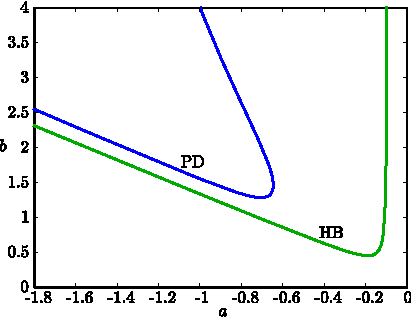
\includegraphics{fig/plot-pd-ns}
\end{center}
\caption{The bifurcation at the Hopf bifurcation curve (HB) is supercritical. 
The periodic solution loses stability at the period doubling bifurcation curve (PD).}
\label{pdbif}
\end{figure}

{ \small \begin{quote} \begin{lstlisting}[basicstyle=\tt,frame=single]
<?xml version="cfile 1.0" encoding="utf-8"?>
<knut version="5"> <branch input="out-start.mat" output="out-nssw.mat"
sysname="mackey-glass.vf" fromtype="NS" label="1"
pointtype="DDE_AUT_HOPF_SW" cp="b" switch="NX" parx="T" nint="80"
ndeg="5" nmul="5" stab="1" curvature="0.25" nint1="12" nint2="12"
ndeg1="4" ndeg2="4" steps="120" iad="3" npr="10" cpmin="-100" cpmax="100"
ds="0.0001" dsmin="0.0001" dsmax="0.005" dsstart="0.0001" epsc="1e-05"
epsr="1e-05" epsk="1e-06" nitc="12" nitr="12" nitk="12" nderi="8" />
</knut>
\end{lstlisting} \end{quote} } \noindent

Checking the the console output, we find that there is a change in
stability between labels 67 and 68, marked by the ``\funp{PD}'' sign referring
to period doubling.
{ \small \begin{quote} \begin{lstlisting}[basicstyle=\tt,frame=single]
IT      ERR             SOLnorm         DIFFnorm
 0      2.881450e-15    8.966784e-01    5.465184e-15

--- Finding the bifurcation point (TF) ---
Re: -6.559948e-01 Im: 7.515199e-01 Angle: 2.288430e+00

IT      ERR             SOLnorm         DIFFnorm
 0      5.294705e-04    8.969029e-01    1.004354e-03
 1      8.039219e-07    8.969027e-01    1.524962e-06

--- Starting the continuation ---
LABEL   NORM           P2             P0             U IT
    0   8.969027E-01   1.336863E+00   2.000000E+00   0  0

Switching to the periodic solution branch at the HOPF point (TF).
SwitchHOPF: T = 5.490064E+00, angle/2PI = 3.642945E-01

LABEL   NORM           P2             P0             U IT
    0   8.969028E-01   1.336864E+00   5.490064E+00   0  2
    1   8.969029E-01   1.336865E+00   5.490065E+00   0  1
    2   8.969032E-01   1.336869E+00   5.490067E+00   0  1 3 2
    3   8.969106E-01   1.336963E+00   5.490117E+00   0  1
    |        |               |             |         |  |
   66   9.141476E-01   1.555239E+00   5.506291E+00   0  2
   67   9.144749E-01   1.559355E+00   5.504824E+00   1  2  PD
   68   9.148008E-01   1.563454E+00   5.503301E+00   1  2 2 2
   69   9.151239E-01   1.567521E+00   5.501730E+00   1  2
\end{lstlisting} \end{quote} } \noindent
This period doubling bifurcation can be continued in two parameters 
by changing the solution type to \funp{12} and including an additional
parameter.
{ \small \begin{quote} \begin{lstlisting}[basicstyle=\tt,frame=single]
<?xml version="cfile 1.0" encoding="utf-8"?>
<knut version="5"> <branch input="out-nssw.mat" output="out-pdsw.mat"
sysname="mackey-glass.vf" fromtype="PD" label="1"
pointtype="DDE_AUT_PD_SW" cp="b" switch="NX" parx="T"
... />
\end{lstlisting} \end{quote} } \noindent
The continuation starts with the following command
{ \small \begin{quote} \begin{lstlisting}[basicstyle=\tt,frame=single]
$ knut -c cfile-pdbif -i in-start
\end{lstlisting} \end{quote} } \noindent
The period doubling curve can be seen in Fig.\ \ref{pdbif}.
Also, the arising period-two orbits can be computed by switching to this new
branch of solutions:
{ \small \begin{quote} \begin{lstlisting}[basicstyle=\tt,frame=single]
<?xml version="cfile 1.0" encoding="utf-8"?>
<knut version="5"> <branch input="out-nssw.mat" output="out-pd.mat"
sysname="mackey-glass.vf" fromtype="PD" label="1" pointtype="DDE_AUT_PD"
cp="b" switch="NX" parx="T,a"
... />
\end{lstlisting} \end{quote} } \noindent
%
\begin{figure}[t!]
\begin{center}
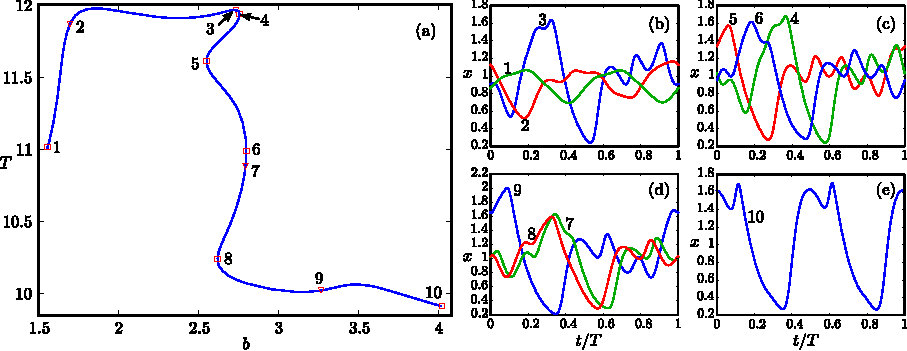
\includegraphics{fig/plot-pdsw}
\end{center}
\caption{The period-two branch (a). Period doublings are denoted by $\bigtriangledown$ and
$\Box$ refers to fold bifurcation. Solution profiles at the bifurcation points are plotted in subfigures (b)-(e).}
\label{pdsw}
\end{figure}
Figure \ref{pdsw} shows the bifurcation diagram of the period-two orbit. Using the
previous methods we continue the bifurcations on this period-two branch, which
gives a more detailed information about the solutions. A three dimensional
bifurcation diagram can be seen in Fig.\ \ref{pdfold}, which shows the
complicated orbit structure.
\begin{figure}[t!]
\begin{center}
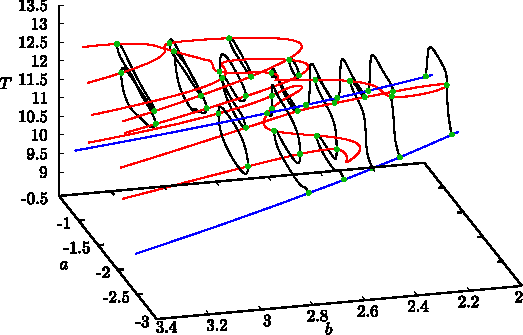
\includegraphics{fig/plot-lp3d}
\end{center}
\caption{Fold bifurcations of the period-two orbits. Black curves are periodic
solutions continued along $b=$constant lines. Red curves refer to fold
bifurcations, and the blue line is the period doubling curve, where the
period-two orbits arise. }
\label{pdfold}
\end{figure}

\section{The graphical user interface (GUI)}

The graphical user interface of the software is a front-end to the computation
library of \knut{}. It can do the same operations as the CLI, however many things are
hidden from the user, so it might appeal to non-expert users. It includes a plotting
facility which can be used to preview the results.

The main window in Fig.\ \ref{mainwindow} appears
when the program \filef{knut-gui} is started.
It has a menu and toolbar which 
contains the \filef{Open} \iconOpen{}, \filef{Save} \iconSave{},
\filef{Run} \iconRun{}, \filef{Stop} \iconStop{} and
\filef{Text} \iconText{} buttons. The \filef{Open} \iconOpen{} button pops up a
file chooser so that an XML-formatted constants file can be chosen. Note that, when opening a constants file an error message will pop up if
the system definition is not compiled yet. To resolve the problem compile the C++ source
of the system definition using the \filef{Compile} \iconBuild{} button and reopen the constants file.

The XML formatted constants file contains the same parameters as the
plain constants file of the CLI, for details see section \ref{constfile}. 
The contents of this XML file can be edited in the four tabs \filef{System},
\filef{Numerics}, \filef{Symmetry} and \filef{Torus} and then can be saved
either using the \filef{Save} \iconSave{} button or the \filef{Save As...}
\iconSaveAs{} menu item in the \filef{File} menu.
\begin{figure}
\begin{center}
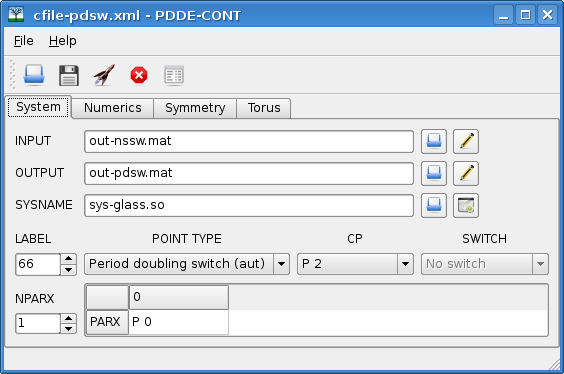
\includegraphics[scale=0.5]{fig/mainwindow}
\caption{The main window of the software. In the toolbar \iconOpen{} opens a constants file, 
\iconSave{} saves the constants file, \iconRun{} starts the continuation, \iconStop{} stops the continuation 
and \iconText{} opens a viewer that contains the same type of output what the command line interface produces. 
There are four tabs: System, Numerics, Symmetry and Torus; these contain the numerical constants. In the line of \filef{INPUT} 
and \filef{OUTPUT} \iconOpen{} opens a {\sc{}mat} file used for obtaining the starting solution and writing 
the results. Toolbutton \iconPencil{} raises a plotting window (see Fig.\ \ref{plotwindow}) that can visualize the results.
In the line of \filef{SYSNAME} \iconOpen{} opens a \filef{sys-problem.so} shared object file and \iconBuild{} compiles 
a system definition file \filef{sys-problem.cpp} . }
\label{mainwindow}
\end{center}
\end{figure}

The \filef{System} tab contains the parameters of the defining system and the
input/output. The \filef{INPUT} and \filef{OUTPUT} labels refer to the input and
output {\sc{}mat} files. These files can be opened using the \filef{Browse} \iconOpen{}
buttons and their contents can be visualized using the \filef{Plot}
\iconPencil{}
buttons. As before, the \filef{LABEL} spinbox contains the solution label in
the input file that is used as a starting point in the numerical continuation.

The system definition file can be selected in the \filef{SYSNAME} line by
opening a shared object (\filef{.so}) file or compiling it from a C++ source
(\filef{.cpp}) file.

The \filef{POINT TYPE} can be selected from the following choices
\begin{itemize}
\item[-] User - user defined equations (not recommended, use
it with symmetric equations only). The equations (\filef{Eqn}) and the
variables (\filef{Var}) have to be selected in the table;
\item[-] Limit cycle - a periodic solution of a forced system, \filef{NPARX}=0. Note that the solution type also can be used to continue equilibria of autonomous systems by keeping the period constant.
\item[-] Limit point - fold bifurcation of a periodic solution in a forced
system, \filef{NPARX}=1;
\item[-] Period doubling - period doubling (flip) bifurcation of a periodic
solution in a forced system, \filef{NPARX}=1;
\item[-] Neimark-Sacker - Neimark-Sacker (secondary Hopf, Torus) bifurcation of
a periodic solution in a forced system, \filef{NPARX}=1;
\item[-] Branch switch - switch to the other branch at a branching point in a
forced system, \filef{NPARX}=0;
\item[-] Period doubling switch - switch to the period-two branch at a period
doubling point in a forced system, \filef{NPARX}=0;
\item[-] Limit cycle (aut)- a periodic solution of a forced system,
\filef{NPARX}=1;
\item[-] Limit point (aut) - fold bifurcation of a periodic solution in an
autonomous system, \filef{NPARX}=2;
\item[-] Period doubling (aut) - period doubling (flip) bifurcation of a
periodic solution in an autonomous system, \filef{NPARX}=2;
\item[-] Neimark-Sacker (aut) - Neimark-Sacker (secondary Hopf, Torus)
bifurcation of a periodic solution in an autonomous system, \filef{NPARX}=2;
\item[-] Branch switch (aut) - switch to the other branch at a branching point
in an autonomous system, \filef{NPARX}=1;
\item[-] Period doubling switch (aut) - switch to the period-two branch at a
period doubling point in an autonomous system, \filef{NPARX}=1;
\item[-] Torus from NS - branch switching from a Neimark-Sacker bifurcation
point to a quasi-periodic torus in a forced system, \filef{NPARX}=1;
\item[-] Torus from NS - branch switching from a Neimark-Sacker bifurcation
point to a quasi-periodic torus in an autonomous, \filef{NPARX}=2;
\end{itemize}
The solution can be continued along the \filef{CP} continuation parameter. If
the \filef{NPARX} parameter is not zero then additional parameter(s)
\filef{PARX} has (have) to be selected from the numbered system parameters
starting with \filef{P} or the two internal parameters the \filef{Rotation
number} (only for tori) and \filef{Angle NS}, which is the argument of the
critical multiplier and can only be selected with the user defined equations.
If the user defined equations are selected it is possible select branch with
the \filef{SWITCH} option.

The \filef{Numerics} tab contains the parameters of the continuation method and
the option of computing stability. For details see section \ref{constfile}.

In the \filef{Symmetry} tab the complex rotational symmetric components of the
solution can be specified. If the parameter \filef{NSYM} is non-zero only the
user defined equations can be used.

The \filef{Torus} tab specifies the mesh parameters of the staggered grid
Chebyshev collocation method when computing quasi-periodic tori.

\subsection{Computing a branch of solutions}

If all the parameters are set up it is recommended to \filef{Save} \iconSave{}
(or \filef{Save as...}) \iconSaveAs{} the settings. To start the computation
press the \filef{Run} \iconRun{} button. Pressing the \filef{Stop} \iconStop{}
button will stop the computation after the approximation of the current point on
the branch is finished.

\subsection{Viewing the results}

The result of the computation can be viewed in textual form. Pressing the
\filef{Text} \iconText{} button in the main window
will pop up the text window (see Fig.\ \ref{textwindow}) that contains almost
the same output as the terminal output of the CLI.
\begin{figure}
\begin{center}
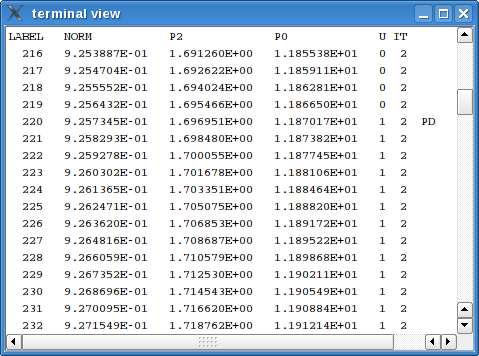
\includegraphics[scale=0.5]{fig/textwindow}
\caption{Textual output view is the same as the command line interface produces. The columns refer to the label,
norm, parameter values, etc.\ of the solution.}
\label{textwindow}
\end{center}
\end{figure}

The solutions branch can also be visualized in a graph in the plotting window (Fig.\
\ref{plotwindow}). If a solution branch is plotted the bifurcation points are
denoted by square, triangle and cross signs in the case of fold, period doubling
and Neimark-Sacker bifurcations, respectively. Note that on Microsoft Windows it is not
possible to plot the results in the middle of a computation. On Linux it is not
a restriction.
\begin{figure}
\begin{center}
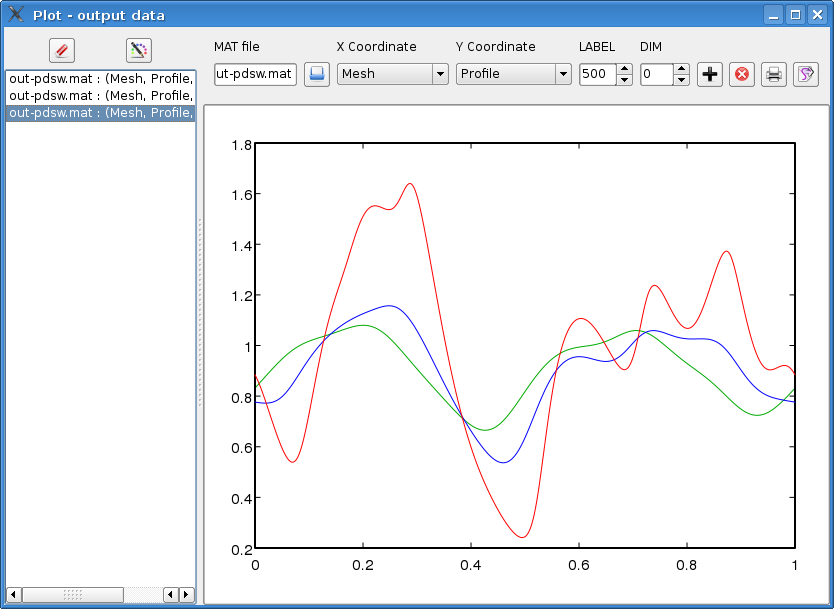
\includegraphics[scale=0.5]{fig/plotwindow}
\caption{The plotting window displays the results of continuation. The {\sc{}mat} file field is the file from where the data is taken.
The X and Y coordinates select the two axis of the planar diagram. If a solution profile is plotted \filef{LABEL} selects the solution 
and \filef{DIM} selects one of its components. Toolbutton \iconAdd{} adds the selected graph to the diagram and 
\iconRemove{} removes all curves from the diagram.
The left side of the window contains the list of curves. If a graph is selected from the list \iconEraser{} removes a graph and \iconColorize{} selects its color.
Keeping the right mouse button pressed the zoom-in area can be selected. Pressing the key P returns to the previous zoom-level.}
\label{plotwindow}
\end{center}
\end{figure}

\section{Algorithms used in the software}

The software uses orthogonal collocation to discretize periodic orbits
\cite{engstab,engcol}. It is also possible to use staggered grid Chebyshev
collocation \cite{kopriva} by changing the collocation and representation points
in \filef{src/ncolloc.cpp}. For continuation, the pseudo arclength method is
used (see, e.g., \cite{handbook, tutorial1, tutorial2}). Codimension-one
bifurcations are computed using the test functionals. The arising bordered
sparse linear systems are solved using the BEMW method developed by Govaerts and
Pryce \cite{Gov1993}. The sparse part of the linear system is factorized by
UMFPACK \cite{umfpack}. Quasiperidic orbits are computed using the spectral
method mentioned above \cite{kopriva,roose-szalai}.

\subsection*{Acknowledgments}

The author is highly indebted to G\'abor St\'ep\'an (Budapest University of 
Technology and Economics) for his constant support. He is also
obliged to S.~John Hogan for partially supporting a 5 month visit at the
University of Bristol.
This research was supported financially by a Hungarian E\"otv\"os Scholarship
and a Fulbright grant.

\appendix

\section{Licenses}

\subsection{KNUT}

In addition to the GNU General Public License below the user of the software or
the author of any
publication containing results obtained using \knut{} or any of its modified
version is required to refer to the present User's Manual.
\begin{quote}
R\'obert Szalai, \knut{}: A continuation and bifurcation software for 
delay-differential equations, Tech.\ Rep., Budapest University of Technology
and Economics (2005)
\end{quote}
In the case of modification of the program please notify the original author and
include a clear description about what was modified and who did the 
modification. Please state clearly that any contribution to this software
contains code which can and will be distributed under the GNU General Public
License.

\begin{quote}
KNUT. A continuation and bifurcation software for delay-differential
equations \\
Copyright (C) 2005 by R\'obert Szalai \\

This program is free software; you can redistribute it and/or modify
it under the terms of the GNU General Public License version 2 as published by
the Free Software Foundation.

This program is distributed in the hope that it will be useful,
but WITHOUT ANY WARRANTY; without even the implied warranty of
MERCHANTABILITY or FITNESS FOR A PARTICULAR PURPOSE.  See the
GNU General Public License for more details.

You should have received a copy of the GNU General Public License
along with this program; if not, write to the Free Software
Foundation, Inc., 51 Franklin Street, Fifth Floor, Boston, MA  02110-1301, USA.
\end{quote}

\subsection{UMFPACK and AMD}

\noindent
UMFPACK Version 4.6, Copyright (c) 2005 by Timothy A. Davis.
All Rights Reserved.
UMFPACK is available under alternate licenses, contact T. Davis for details.\\
\url{http://www.cise.ufl.edu/research/sparse/umfpack}\\
Your use or distribution of UMFPACK or any modified version of
UMFPACK implies that you agree to this License.

\noindent
AMD Version 1.1 (Jan. 10, 2004),
Copyright (c) 2004 by Timothy A.~Davis, Patrick R.~Amestoy, and Iain S.~Duff.
All Rights Reserved.\\
\url{http://www.cise.ufl.edu/research/sparse/amd}\\
Your use or distribution of AMD or any modified version of
AMD implies that you agree to this License.

UMFPACK and AMD License:
\begin{quote}
    This library is free software; you can redistribute it and/or
    modify it under the terms of the GNU Lesser General Public
    License as published by the Free Software Foundation; either
    version 2.1 of the License, or (at your option) any later version.

    This library is distributed in the hope that it will be useful,
    but WITHOUT ANY WARRANTY; without even the implied warranty of
    MERCHANTABILITY or FITNESS FOR A PARTICULAR PURPOSE.  See the GNU
    Lesser General Public License for more details.

    You should have received a copy of the GNU Lesser General Public
    License along with this library; if not, write to the Free Software
    Foundation, Inc., 51 Franklin St, Fifth Floor, Boston, MA  02110-1301
    USA

    Permission is hereby granted to use or copy this program under the
    terms of the GNU LGPL, provided that the Copyright, this License,
    and the Availability of the original version is retained on all copies.
    User documentation of any code that uses this code or any modified
    version of this code must cite the Copyright, this License, the
    Availability note, and "Used by permission." Permission to modify
    the code and to distribute modified code is granted, provided the
    Copyright, this License, and the Availability note are retained,
    and a notice that the code was modified is included.
\end{quote}

\bibliographystyle{plain}
\bibliography{manual-bibl.bib} \label{sec:bibliography}


\end{document}
